\documentclass[12pt]{article}
\usepackage[utf8]{inputenc}
\usepackage[letterpaper, margin=1in]{geometry}
\usepackage[dvipsnames]{xcolor}
\usepackage{graphicx}
\usepackage{subcaption}
\graphicspath{{./figures/}}
\usepackage{hyperref}
\hypersetup{
    colorlinks=true,   
    urlcolor=blue,
}
\usepackage{parskip}
\usepackage{amsmath}
\usepackage{titlesec}
\usepackage{listings}

\definecolor{backgroundColour}{rgb}{0.95,0.95,0.92}
\lstset{
    % frame=single,
    captionpos=t,   % sets the caption-position to top
    breaklines=true,
    numbers=left,
    % numbersep=5pt,
    numberstyle=\tiny\color{gray},
    tabsize=2,
    basicstyle=\ttfamily\scriptsize,
    showspaces=false,
    showstringspaces=false,
    backgroundcolor=\color{backgroundColour},
    keywordstyle=\color{Magenta},
    identifierstyle=\color{MidnightBlue},
    commentstyle=\color{Green},
    stringstyle=\color{Maroon}}


\titleformat*{\section}{\large\bfseries}
%\allowdisplaybreaks

% remove vertical spacing above top figure
\makeatletter
\setlength{\@fptop}{0pt}
\makeatother
%

\title{COMPENG 4DS4 Lab 2 Report}
\author{
    Aaron Pinto \\
    pintoa9 \\
    \and
    Raeed Hassan \\
    hassam41 \\
    \and
    Jingming Liu \\
    liuj171 \\
    \and
    Jeffrey Guo \\
    guoj69 \\
}

\begin{document}

\maketitle
\clearpage

\section*{Declaration of Contributions}
\begin{table}[htp]
\centering
\begin{tabular}{|l|l|}
\hline
    Problem & Contributions             \\ \hline
    1       & Aaron, Jeffrey            \\ \hline
    2       & Aaron, Raeed              \\ \hline
    3       & Aaron, Jingming           \\ \hline
    4       & Jingming, Raeed           \\ \hline
    5       & Jingming, Raeed           \\ \hline
    6       & Jingming, Raeed           \\ \hline
    7       & Jingming, Raeed           \\ \hline
\end{tabular}
\end{table}
\clearpage

\section*{Problem 1}
The code listing for problem 1 is Listing~\ref{list:p1}. The \texttt{MEM\_LOC} macro was redefined for the different sizes we required (\texttt{MEM\_LOC\_CHAR} for 1 byte, \texttt{MEM\_LOC\_SHORT} for 2 bytes, and \texttt{MEM\_LOC\_INT} for 4 bytes). The required addresses were defined in the macros \texttt{LOC1}-\texttt{LOC4}, using the new macros created for \texttt{MEM\_LOC}. These macros are used in the function \texttt{problem1} to write the required values to the memory addresses.

The memory and expression panels for problem 1 are shown in Figure~\ref{fig:p1}. The endianness was set to big, the cell size to 1 byte, and the radix to hex.

\begin{lstlisting}[language=c,caption=Problem 1, label=list:p1]
/* Definitions */
#define MEM_LOC_CHAR(x)             *((char*)x)
#define MEM_LOC_SHORT(x)            *((short*)x)
#define MEM_LOC_INT(x)              *((int*)x)
#define LOC1                        MEM_LOC_CHAR(0x20001000)
#define LOC2                        MEM_LOC_INT(0x20001001)
#define LOC3                        MEM_LOC_SHORT(0x20001005)
#define LOC4                        MEM_LOC_INT(0x20001007)

/* Problem 1 Function */
void problem1() {
    LOC1 = 0xAC;
    LOC2 = 0xAABBCCDD;
    LOC3 = 0xABCD;
    LOC4 = 0xAABBCCDD;
}
\end{lstlisting}

\begin{figure}[htp]
\centering
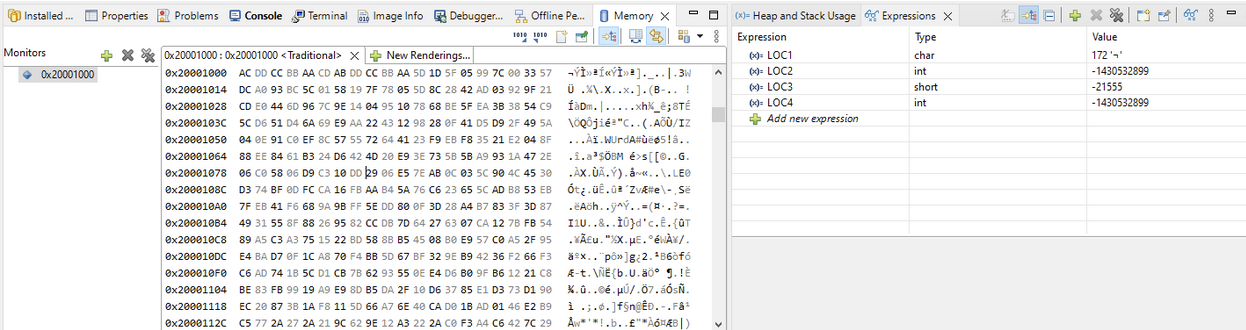
\includegraphics[width=\textwidth]{p1}
\caption[problem 1]{Memory and Expression Panels for Problem 1}\label{fig:p1}
\end{figure}
\begin{filecontents}[overwrite]{./sections/p2_main.tex}
\begin{lstlisting}[language=c,caption=Problem 2 main, label=list:p2_main]
int main(void) {
    BaseType_t status;
    /* Init board hardware. */
    BOARD_InitBootPins();
    BOARD_InitBootClocks();
    BOARD_InitDebugConsole();

    queue1 = xQueueCreate(10, sizeof(char*));

    if (queue1 == NULL) {
        PRINTF("Queue creation failed!.\r\n");
        while (1)
            ;
    }

    status = xTaskCreate(producer_queue, "producer", 200, (void*) queue1, 2, NULL);
    if (status != pdPASS) {
        PRINTF("Task creation failed!.\r\n");
        while (1)
            ;
    }

    status = xTaskCreate(consumer_queue, "consumer", 200, (void*) queue1, 3, NULL);
    if (status != pdPASS) {
        PRINTF("Task creation failed!.\r\n");
        while (1)
            ;
    }

    vTaskStartScheduler();

    while (1) {
    }

}
\end{lstlisting}
\end{filecontents}

\begin{filecontents}[overwrite]{./sections/p2_producer.tex}
\begin{lstlisting}[language=c,caption=Problem 2 Producer Queue, label=list:p2_prod]
void producer_queue(void *pvParameters) {
    QueueHandle_t queue1 = (QueueHandle_t) pvParameters;
    BaseType_t status;

    char *usr_str;
    usr_str = malloc(sizeof(char) * 10);

    printf("please enter a string\n");
    scanf("%s", usr_str);

    while (1) {
        status = xQueueSend(queue1, (void* ) &usr_str, portMAX_DELAY);
        if (status != pdPASS) {
            PRINTF("Queue Send failed!.\r\n");
            while (1)
                ;
        }

        vTaskDelay(1000 / portTICK_PERIOD_MS);
    }

    vTaskDelete(NULL);
}
\end{lstlisting}
\end{filecontents}


\begin{filecontents}[overwrite]{./sections/p2_consumer.tex}
\begin{lstlisting}[language=c,caption=Problem 2 Consumer Queue, label=list:p2_cons]
void consumer_queue(void *pvParameters) {
    QueueHandle_t queue1 = (QueueHandle_t) pvParameters;
    BaseType_t status;

    char *receive_str;

    while (1) {
        status = xQueueReceive(queue1, (void*) &receive_str, portMAX_DELAY);

        if (status != pdPASS) {
            PRINTF("Queue Receive failed!.\r\n");

            while (1)
                ;
        }

        PRINTF("Received Value = %s\r\n", receive_str);
    }
}    
\end{lstlisting}
\end{filecontents}

\section*{Problem 2}
When repeating Problem 1 with queues, we have a producer task handling the user input and a consumer task printing the string. The priority of the producer is 2 and the consumer is 3. The queue declared is \texttt{queue1}. In the producer task, the user input \texttt{usr\_str} will be put in the queue by \texttt{xQueueSend}. The consumer task is blocked by \texttt{xQueueReceive} until producer one sends the input string, which will also be received by \texttt{xQueueReceive}. After the string is received on the consumer side, it will be printed to the console.

The main function is shown below in Listing~\ref{list:p2_main}. The two tasks are shown in Listings~\ref{list:p2_prod} and \ref{list:p2_cons}.

%% LaTeX2e file `./sections/p2_main.tex'
%% generated by the `filecontents' environment
%% from source `lab2' on 2023/03/03.
%%
\begin{lstlisting}[language=c,caption=Problem 2 main, label=list:p2_main]
int main(void) {
    BaseType_t status;
    /* Init board hardware. */
    BOARD_InitBootPins();
    BOARD_InitBootClocks();
    BOARD_InitDebugConsole();

    queue1 = xQueueCreate(10, sizeof(char*));

    if (queue1 == NULL) {
        PRINTF("Queue creation failed!.\r\n");
        while (1)
            ;
    }

    status = xTaskCreate(producer_queue, "producer", 200, (void*) queue1, 2, NULL);
    if (status != pdPASS) {
        PRINTF("Task creation failed!.\r\n");
        while (1)
            ;
    }

    status = xTaskCreate(consumer_queue, "consumer", 200, (void*) queue1, 3, NULL);
    if (status != pdPASS) {
        PRINTF("Task creation failed!.\r\n");
        while (1)
            ;
    }

    vTaskStartScheduler();

    while (1) {
    }

}
\end{lstlisting}

%% LaTeX2e file `./sections/p2_producer.tex'
%% generated by the `filecontents' environment
%% from source `lab2' on 2023/03/03.
%%
\begin{lstlisting}[language=c,caption=Problem 2 Producer Queue, label=list:p2_prod]
void producer_queue(void *pvParameters) {
    QueueHandle_t queue1 = (QueueHandle_t) pvParameters;
    BaseType_t status;

    char *usr_str;
    usr_str = malloc(sizeof(char) * 10);

    printf("please enter a string\n");
    scanf("%s", usr_str);

    while (1) {
        status = xQueueSend(queue1, (void* ) &usr_str, portMAX_DELAY);
        if (status != pdPASS) {
            PRINTF("Queue Send failed!.\r\n");
            while (1)
                ;
        }

        vTaskDelay(1000 / portTICK_PERIOD_MS);
    }

    vTaskDelete(NULL);
}
\end{lstlisting}

%% LaTeX2e file `./sections/p2_consumer.tex'
%% generated by the `filecontents' environment
%% from source `lab2' on 2023/03/03.
%%
\begin{lstlisting}[language=c,caption=Problem 2 Consumer Queue, label=list:p2_cons]
void consumer_queue(void *pvParameters) {
    QueueHandle_t queue1 = (QueueHandle_t) pvParameters;
    BaseType_t status;

    char *receive_str;

    while (1) {
        status = xQueueReceive(queue1, (void*) &receive_str, portMAX_DELAY);

        if (status != pdPASS) {
            PRINTF("Queue Receive failed!.\r\n");

            while (1)
                ;
        }

        PRINTF("Received Value = %s\r\n", receive_str);
    }
}
\end{lstlisting}

\section*{Problem 3}
The code listing for problem 3 is Listing~\ref{list:p3}. The \texttt{BOARD\_InitPins} function was updated to initialize the appropriate GPIO ports and pins (GPIOC 8 and 9 for blue and green, GPIOD 1 for red). The \texttt{GPIO\_PinInit} and \texttt{GPIO\_PortToggle} functions provided in the example were used to initialize the LEDs to an OFF state and for toggling the LEDs in the while loop.

\begin{lstlisting}[language=c,caption=Problem 3, label=list:p3]
/* Definitions */
#define BOARD_LED_GPIO_BLUE         GPIOC
#define BOARD_LED_GPIO_PIN_BLUE     8
#define BOARD_LED_GPIO_GREEN        GPIOC
#define BOARD_LED_GPIO_PIN_GREEN    9
#define BOARD_LED_GPIO_RED          GPIOD
#define BOARD_LED_GPIO_PIN_RED      1

/* BOARD_InitPins function */
void BOARD_InitPins(void) {
    /* Port C Clock Gate Control: Clock enabled */
    CLOCK_EnableClock(kCLOCK_PortC);
    /* Port D Clock Gate Control: Clock enabled */
    CLOCK_EnableClock(kCLOCK_PortD);

    /* PORTC8 is configured as PTC8 */
    PORT_SetPinMux(PORTC, 8U, kPORT_MuxAsGpio);

    /* PORTC9 is configured as PTC9 */
    PORT_SetPinMux(PORTC, 9U, kPORT_MuxAsGpio);

    /* PORTD1 is configured as PTD1 */
    PORT_SetPinMux(PORTD, 1U, kPORT_MuxAsGpio);
}


/* Problem 3 main Function */
int main(void) {
    /* Define the init structure for the output LED pin*/
    gpio_pin_config_t led_config = {kGPIO_DigitalOutput, 0};

    /* Board pin, clock, debug console init */
    BOARD_InitBootPins();
    BOARD_InitBootClocks();
    BOARD_InitDebugConsole();

    /* Print a note to terminal. */
    PRINTF("\r\n GPIO Driver example\r\n");
    PRINTF("\r\n The LED is blinking.\r\n");

    /* Init output LED GPIO. */
    GPIO_PinInit(BOARD_LED_GPIO_BLUE, BOARD_LED_GPIO_PIN_BLUE, &led_config);
    GPIO_PinInit(BOARD_LED_GPIO_GREEN, BOARD_LED_GPIO_PIN_GREEN, &led_config);
    GPIO_PinInit(BOARD_LED_GPIO_RED, BOARD_LED_GPIO_PIN_RED, &led_config);

    while (1) {
        delay();
        GPIO_PortToggle(BOARD_LED_GPIO_BLUE, 1u << BOARD_LED_GPIO_PIN_BLUE);
        delay();
        GPIO_PortToggle(BOARD_LED_GPIO_BLUE, 1u << BOARD_LED_GPIO_PIN_BLUE);
        delay();
        GPIO_PortToggle(BOARD_LED_GPIO_GREEN, 1u << BOARD_LED_GPIO_PIN_GREEN);
        delay();
        GPIO_PortToggle(BOARD_LED_GPIO_GREEN, 1u << BOARD_LED_GPIO_PIN_GREEN);
        delay();
        GPIO_PortToggle(BOARD_LED_GPIO_RED, 1u << BOARD_LED_GPIO_PIN_RED);
        delay();
        GPIO_PortToggle(BOARD_LED_GPIO_RED, 1u << BOARD_LED_GPIO_PIN_RED);
    }
}
\end{lstlisting}
\section*{Problem 4}
The code listing for Problem 4, the \texttt{SPI\_write} function, is Listing~\ref{list:p4_spi_write}. The function is mostly a duplicate of the provided \texttt{SPI\_read} function. It changes the initialized sizes of \texttt{masterTxData} and \texttt{masterRxData} to always be 3 bytes as we are only writing 1 byte of data, and two additional bytes are required to select between READ or WRITE and to select the register address.

As outlined in the FXOS8700CQ documentation, we set the value of R/W to 1 for write. The order of bits for a write operation is as follows:\\
Byte 0: R/W,ADDR[6],ADDR[5],ADDR[4],ADDR[3],ADDR[2],ADDR[1],ADDR[0],\\
Byte 1: ADDR[7],X,X,X,X,X,X,X,\\
Byte 2: DATA[7],DATA[6],DATA[5],DATA[4],DATA[3],DATA[2],DATA[1],DATA[0].
\begin{lstlisting}[language=c,caption=Problem 4 SPI\_write, label=list:p4_spi_write]
status_t SPI_write(uint8_t regAddress, uint8_t value)
{
    dspi_transfer_t masterXfer;
    uint8_t *masterTxData = (uint8_t *)malloc(3);
    uint8_t *masterRxData = (uint8_t *)malloc(3);

    masterTxData[0] = regAddress | 0x80; // Sets the most significant bit (enable write)
    masterTxData[1] = regAddress & 0x80; // Clear the least significant 7 bits
    masterTxData[2] = value;

    masterXfer.txData = masterTxData;
    masterXfer.rxData = masterRxData;
    masterXfer.dataSize = 3;
    masterXfer.configFlags = kDSPI_MasterCtar0 | kDSPI_MasterPcs0 | kDSPI_MasterPcsContinuous;
    status_t ret = DSPI_MasterTransferBlocking(SPI1, &masterXfer);

    free(masterTxData);
    free(masterRxData);

    return ret;
}
\end{lstlisting}

The main function is shown below in Listing~\ref{list:p4_main}. We test our function with the PL\_COUNT register since it has 8 bits available for both read and write. The register is also available for both read and write during active mode. After the write, we read the value of the register by SPI and the register value changed as we wanted.
\begin{lstlisting}[language=c,caption=Problem 4 main, label=list:p4_main]
int main(void)
{
    uint8_t byte;
    uint8_t write_test_byte = 0xCC;
    uint8_t read_test_byte;

    /* Init board hardware. */
    BOARD_InitBootPins();
    BOARD_InitBootClocks();

    voltageRegulatorEnable();
    accelerometerEnable();
    
    setupSPI();
    
    /******* Delay *******/
    for (volatile int i = 0U; i < 1000000; i++)
        __asm("NOP");
    
    SPI_read(0x0D, &byte, 1);
    printf("The expected value is 0xC7 and the read value 0x%X\n", byte);
    
    printf("reading  to the PL_COUNT register  before writing \n");
    SPI_read(0x12, &read_test_byte, 1);
    printf("The expected value for PL_COUNT register is 0x0 and the read value 0x%X\n", read_test_byte);

    SPI_write(0x12, write_test_byte);
    printf("writing to the PL_COUNT register \n");

    SPI_read(0x12, &read_test_byte, 1);
    printf("The expected value for the PL_COUNT register is 0xCC and the read value 0x%X\n", read_test_byte);

    while (1)
    {
    }
}
\end{lstlisting}
\section*{Problem 5}
The code listing for problem 5 is split between Listing~\ref{list:p5_ftm} for the FTM/PWM setup, and Listing~\ref{list:p5_main} for the \texttt{main} function.

In the FTM setup, we update the \texttt{pwm\_setup} function provided in the lab to include the FTM setup for \texttt{UI\_LED\_GREEN} and \texttt{UI\_LED\_BLUE}. The appropriate alternative functions to output PWM signals for these GPIO pins were documented in the datasheet.
\begin{lstlisting}[language=c,caption=Problem 5 FTM/PWM Setup, label=list:p5_ftm]
void pwm_setup() {
    ftm_config_t ftmInfo;
    ftm_chnl_pwm_signal_param_t ftmParam;
    
    /* UI_LED_RED PWM Setup */
    ftmParam.chnlNumber = kFTM_Chnl_1;
    ftmParam.level = kFTM_HighTrue;
    ftmParam.dutyCyclePercent = 0;
    ftmParam.firstEdgeDelayPercent = 0U;
    ftmParam.enableComplementary = false;
    ftmParam.enableDeadtime = false;

    FTM_GetDefaultConfig(&ftmInfo);

    FTM_Init(FTM3, &ftmInfo);
    FTM_SetupPwm(FTM3, &ftmParam, 1U, kFTM_EdgeAlignedPwm, 5000U, CLOCK_GetFreq(kCLOCK_BusClk));
    FTM_StartTimer(FTM3, kFTM_SystemClock);
    
    /* UI_LED_BLUE PWM Setup */
    ftmParam.chnlNumber = kFTM_Chnl_4;
    ftmParam.level = kFTM_HighTrue;
    ftmParam.dutyCyclePercent = 0;
    ftmParam.firstEdgeDelayPercent = 0U;
    ftmParam.enableComplementary = false;
    ftmParam.enableDeadtime = false;

    FTM_GetDefaultConfig(&ftmInfo);

    FTM_Init(FTM3, &ftmInfo);
    FTM_SetupPwm(FTM3, &ftmParam, 1U, kFTM_EdgeAlignedPwm, 5000U, CLOCK_GetFreq(kCLOCK_BusClk));
    FTM_StartTimer(FTM3, kFTM_SystemClock);

    /* UI_LED_GREEN PWM Setup */
    ftmParam.chnlNumber = kFTM_Chnl_5;
    ftmParam.level = kFTM_HighTrue;
    ftmParam.dutyCyclePercent = 0;
    ftmParam.firstEdgeDelayPercent = 0U;
    ftmParam.enableComplementary = false;
    ftmParam.enableDeadtime = false;

    FTM_GetDefaultConfig(&ftmInfo);

    FTM_Init(FTM3, &ftmInfo);
    FTM_SetupPwm(FTM3, &ftmParam, 1U, kFTM_EdgeAlignedPwm, 5000U, CLOCK_GetFreq(kCLOCK_BusClk));
    FTM_StartTimer(FTM3, kFTM_SystemClock);
}
\end{lstlisting}

The \texttt{main} function provided in the lab was modified to include the PWM functions to update \texttt{UI\_LED\_GREEN} and \texttt{UI\_LED\_BLUE}. The \texttt{scanf} was modified to read in 6 characters and store each two character inputs as two hexadecimal characters in variables corresponding to the duty cycle for the red, green, and blue LEDs. The percent value of these inputs (out of 0xFF) are calculated as the \texttt{FTM\_UpdatePwmDutycycle} function requires the duty cycle to be an \texttt{uint8\_t} between 0 and 100 representing the duty cycle percentage.
\begin{lstlisting}[language=c,caption=Problem 5 main, label=list:p5_main]
int main(void) {
    unsigned int duty_cycle_red = 0;
    unsigned int duty_cycle_green = 0;
    unsigned int duty_cycle_blue = 0;

    /* Init board hardware. */
    BOARD_InitBootPins();
    BOARD_InitBootClocks();
    BOARD_InitDebugConsole();

    pwm_setup();

    scanf("%2x%2x%2x", &duty_cycle_red, &duty_cycle_green, &duty_cycle_blue);

    printf("red = %x\n", duty_cycle_red);
    printf("green = %x\n", duty_cycle_green);
    printf("blue = %x\n", duty_cycle_blue);

    float red = (duty_cycle_red / 255.0) * 100;
    float green = (duty_cycle_green / 255.0) * 100;
    float blue = (duty_cycle_blue / 255.0) * 100;

    FTM_UpdatePwmDutycycle(FTM3, kFTM_Chnl_1, kFTM_EdgeAlignedPwm, (uint8_t)red);
    FTM_SetSoftwareTrigger(FTM3, true);

    FTM_UpdatePwmDutycycle(FTM3, kFTM_Chnl_5, kFTM_EdgeAlignedPwm, (uint8_t)green);
    FTM_SetSoftwareTrigger(FTM3, true);

    FTM_UpdatePwmDutycycle(FTM3, kFTM_Chnl_4, kFTM_EdgeAlignedPwm, (uint8_t)blue);
    FTM_SetSoftwareTrigger(FTM3, true);

    while (1) {
    }
}
\end{lstlisting}
% \begin{filecontents}[overwrite]{./sections/p6_main.tex}
\begin{lstlisting}[language=c,caption=Problem 6 Producer Task, label=list:p6_main]
int main(void) {
    BaseType_t status;
    /* Init board hardware. */
    BOARD_InitBootPins();
    BOARD_InitBootClocks();
    BOARD_InitDebugConsole();

    semaphores = (SemaphoreHandle_t*) malloc(1 * sizeof(SemaphoreHandle_t));
    semaphores[0] = xSemaphoreCreateBinary(); // Consumer semaphore

    status = xTaskCreate(consumer_sem, "consumer", 200, (void*) semaphores, 2, NULL);
    if (status != pdPASS) {
        PRINTF("Task creation failed!.\r\n");
        while (1)
            ;
    }

    TimerHandle_t timer_handle2 = xTimerCreate("Periodic timer",
            1000 / portTICK_PERIOD_MS,
            pdTRUE,
            NULL, timerCallbackFunction2);

    status = xTimerStart(timer_handle2, 0);
    if (status != pdPASS) {
        PRINTF("Couldn't start the timer!.\r\n");
        while (1)
            ;
    }

    vTaskStartScheduler();
    while (1) {
    }
}
\end{lstlisting}
\end{filecontents}

\begin{filecontents}[overwrite]{./sections/p6_timer.tex}
\begin{lstlisting}[language=c,caption=Problem 6 Periodic Timer Callback Function, label=list:p6_timer]
void timerCallbackFunction2(TimerHandle_t timer_handle) {
    SemaphoreHandle_t consumer_semaphore = semaphores[0];
    BaseType_t status;

    xSemaphoreGive(consumer_semaphore);
}
\end{lstlisting}
\end{filecontents}

\begin{filecontents}[overwrite]{./sections/p6_print.tex}
\begin{lstlisting}[language=c,caption=Problem 6 Print Task, label=list:p6_print]
void consumer_sem(void *pvParameters) {
    SemaphoreHandle_t consumer_semaphore = semaphores[0];
    BaseType_t status;

    while (1) {
        status = xSemaphoreTake(consumer_semaphore, portMAX_DELAY);
        if (status != pdPASS) {
            PRINTF("Failed to acquire consumer_semaphore\r\n");
            while (1)
                ;
        }

        PRINTF("Hello World!\n");
    }
}
\end{lstlisting}
\end{filecontents}

\section*{Problem 6}
We create a periodic timer with the callback function defined in \texttt{timerCallbackFunction2}. The timer callback function signals a semaphore every second. The task will block on \texttt{xSemaphoreTake} until it receives a signal from the semaphore, then print a message on the console.

The main function is shown below in Listing~\ref{list:p6_main}. The timer callback function is shown in Listing~\ref{list:p6_timer}. The print task is shown in Listing~\ref{list:p6_print}.

%% LaTeX2e file `./sections/p6_main.tex'
%% generated by the `filecontents' environment
%% from source `lab2' on 2023/03/03.
%%
\begin{lstlisting}[language=c,caption=Problem 6 Producer Task, label=list:p6_main]
int main(void) {
    BaseType_t status;
    /* Init board hardware. */
    BOARD_InitBootPins();
    BOARD_InitBootClocks();
    BOARD_InitDebugConsole();

    semaphores = (SemaphoreHandle_t*) malloc(1 * sizeof(SemaphoreHandle_t));
    semaphores[0] = xSemaphoreCreateBinary(); // Consumer semaphore

    status = xTaskCreate(consumer_sem, "consumer", 200, (void*) semaphores, 2, NULL);
    if (status != pdPASS) {
        PRINTF("Task creation failed!.\r\n");
        while (1)
            ;
    }

    TimerHandle_t timer_handle2 = xTimerCreate("Periodic timer",
            1000 / portTICK_PERIOD_MS,
            pdTRUE,
            NULL, timerCallbackFunction2);

    status = xTimerStart(timer_handle2, 0);
    if (status != pdPASS) {
        PRINTF("Couldn't start the timer!.\r\n");
        while (1)
            ;
    }

    vTaskStartScheduler();
    while (1) {
    }
}
\end{lstlisting}

%% LaTeX2e file `./sections/p6_timer.tex'
%% generated by the `filecontents' environment
%% from source `lab2' on 2023/03/03.
%%
\begin{lstlisting}[language=c,caption=Problem 6 Periodic Timer Callback Function, label=list:p6_timer]
void timerCallbackFunction2(TimerHandle_t timer_handle) {
    SemaphoreHandle_t consumer_semaphore = semaphores[0];
    BaseType_t status;

    xSemaphoreGive(consumer_semaphore);
}
\end{lstlisting}

%% LaTeX2e file `./sections/p6_print.tex'
%% generated by the `filecontents' environment
%% from source `lab2' on 2023/03/03.
%%
\begin{lstlisting}[language=c,caption=Problem 6 Print Task, label=list:p6_print]
void consumer_sem(void *pvParameters) {
    SemaphoreHandle_t consumer_semaphore = semaphores[0];
    BaseType_t status;

    while (1) {
        status = xSemaphoreTake(consumer_semaphore, portMAX_DELAY);
        if (status != pdPASS) {
            PRINTF("Failed to acquire consumer_semaphore\r\n");
            while (1)
                ;
        }

        PRINTF("Hello World!\n");
    }
}
\end{lstlisting}


% \section*{Problem 7}
The variable \texttt{rc\_values} contains a structure \texttt{RC\_Values}, which stores 9 2-byte integers, one integer for the header and eight integers for each of the eight data channel. This structure is used to store the data received via UART.

The variable \texttt{ptr} contains a pointer to the address of \texttt{rc\_values}, specifically the address to the first byte of \texttt{rc\_values}. When the main function is run and a stream of data is received via UART, the first byte is checked and stored in \texttt{ptr}, or the first byte of \texttt{rc\_values}. The value of this byte is checked to see if matches \texttt{0x20}, which is the first expected byte of data stream received. If this matches, the remaining 17 bytes are read via UART and stored at \texttt{\&ptr[1]}, which points to the address of the second byte of \texttt{header} in the structure.
\end{document}